\ifx\fulldocument\undefined
\documentclass[aspectratio=169]{beamer}
% \usetheme{sdr}
\graphicspath{{./tex/imgs/}}

\usepackage[utf8]{inputenc}

\title{Programmiamo Umanoidi!}
\subtitle{}
\author{Lorenzo Leonardini}
\institute{Scuola di Robotica}
\date{\today}

\begin{document}

\begin{frame}
	\titlepage
\end{frame}

\section{Che cos'è NAO}
\subsection{Caratteristiche}
\subsection{Movimento}
\subsection{Utilizzi}
\subsection{Software}
\section{Choregraphe}
\section{Primo programma}
\section{NAO Actor Studio}

\AtBeginSection[]
{
\begin{frame}{Indice}
\tableofcontents[currentsection]
\end{frame}
}
\fi

\section{NAO In The Store}

\begin{frame}
\frametitle{NAO In The Store}
\begin{columns}
	\column{0.5\textwidth}
		\begin{itemize}
			\item<1->Si stanno diffondendo sempre di più assistenti vocali e robotici
			\item<2->Amazon Alexa, Google Home...
			\item<3->I robot raggiungono i negozi: Pepper
			\item<4->Negozi di telefonia in Giappone, negozi al dettaglio in America, concessionario a Brescia
		\end{itemize}
	\column{0.5\textwidth}
		\begin{figure}[ht]
		\begin{center}
		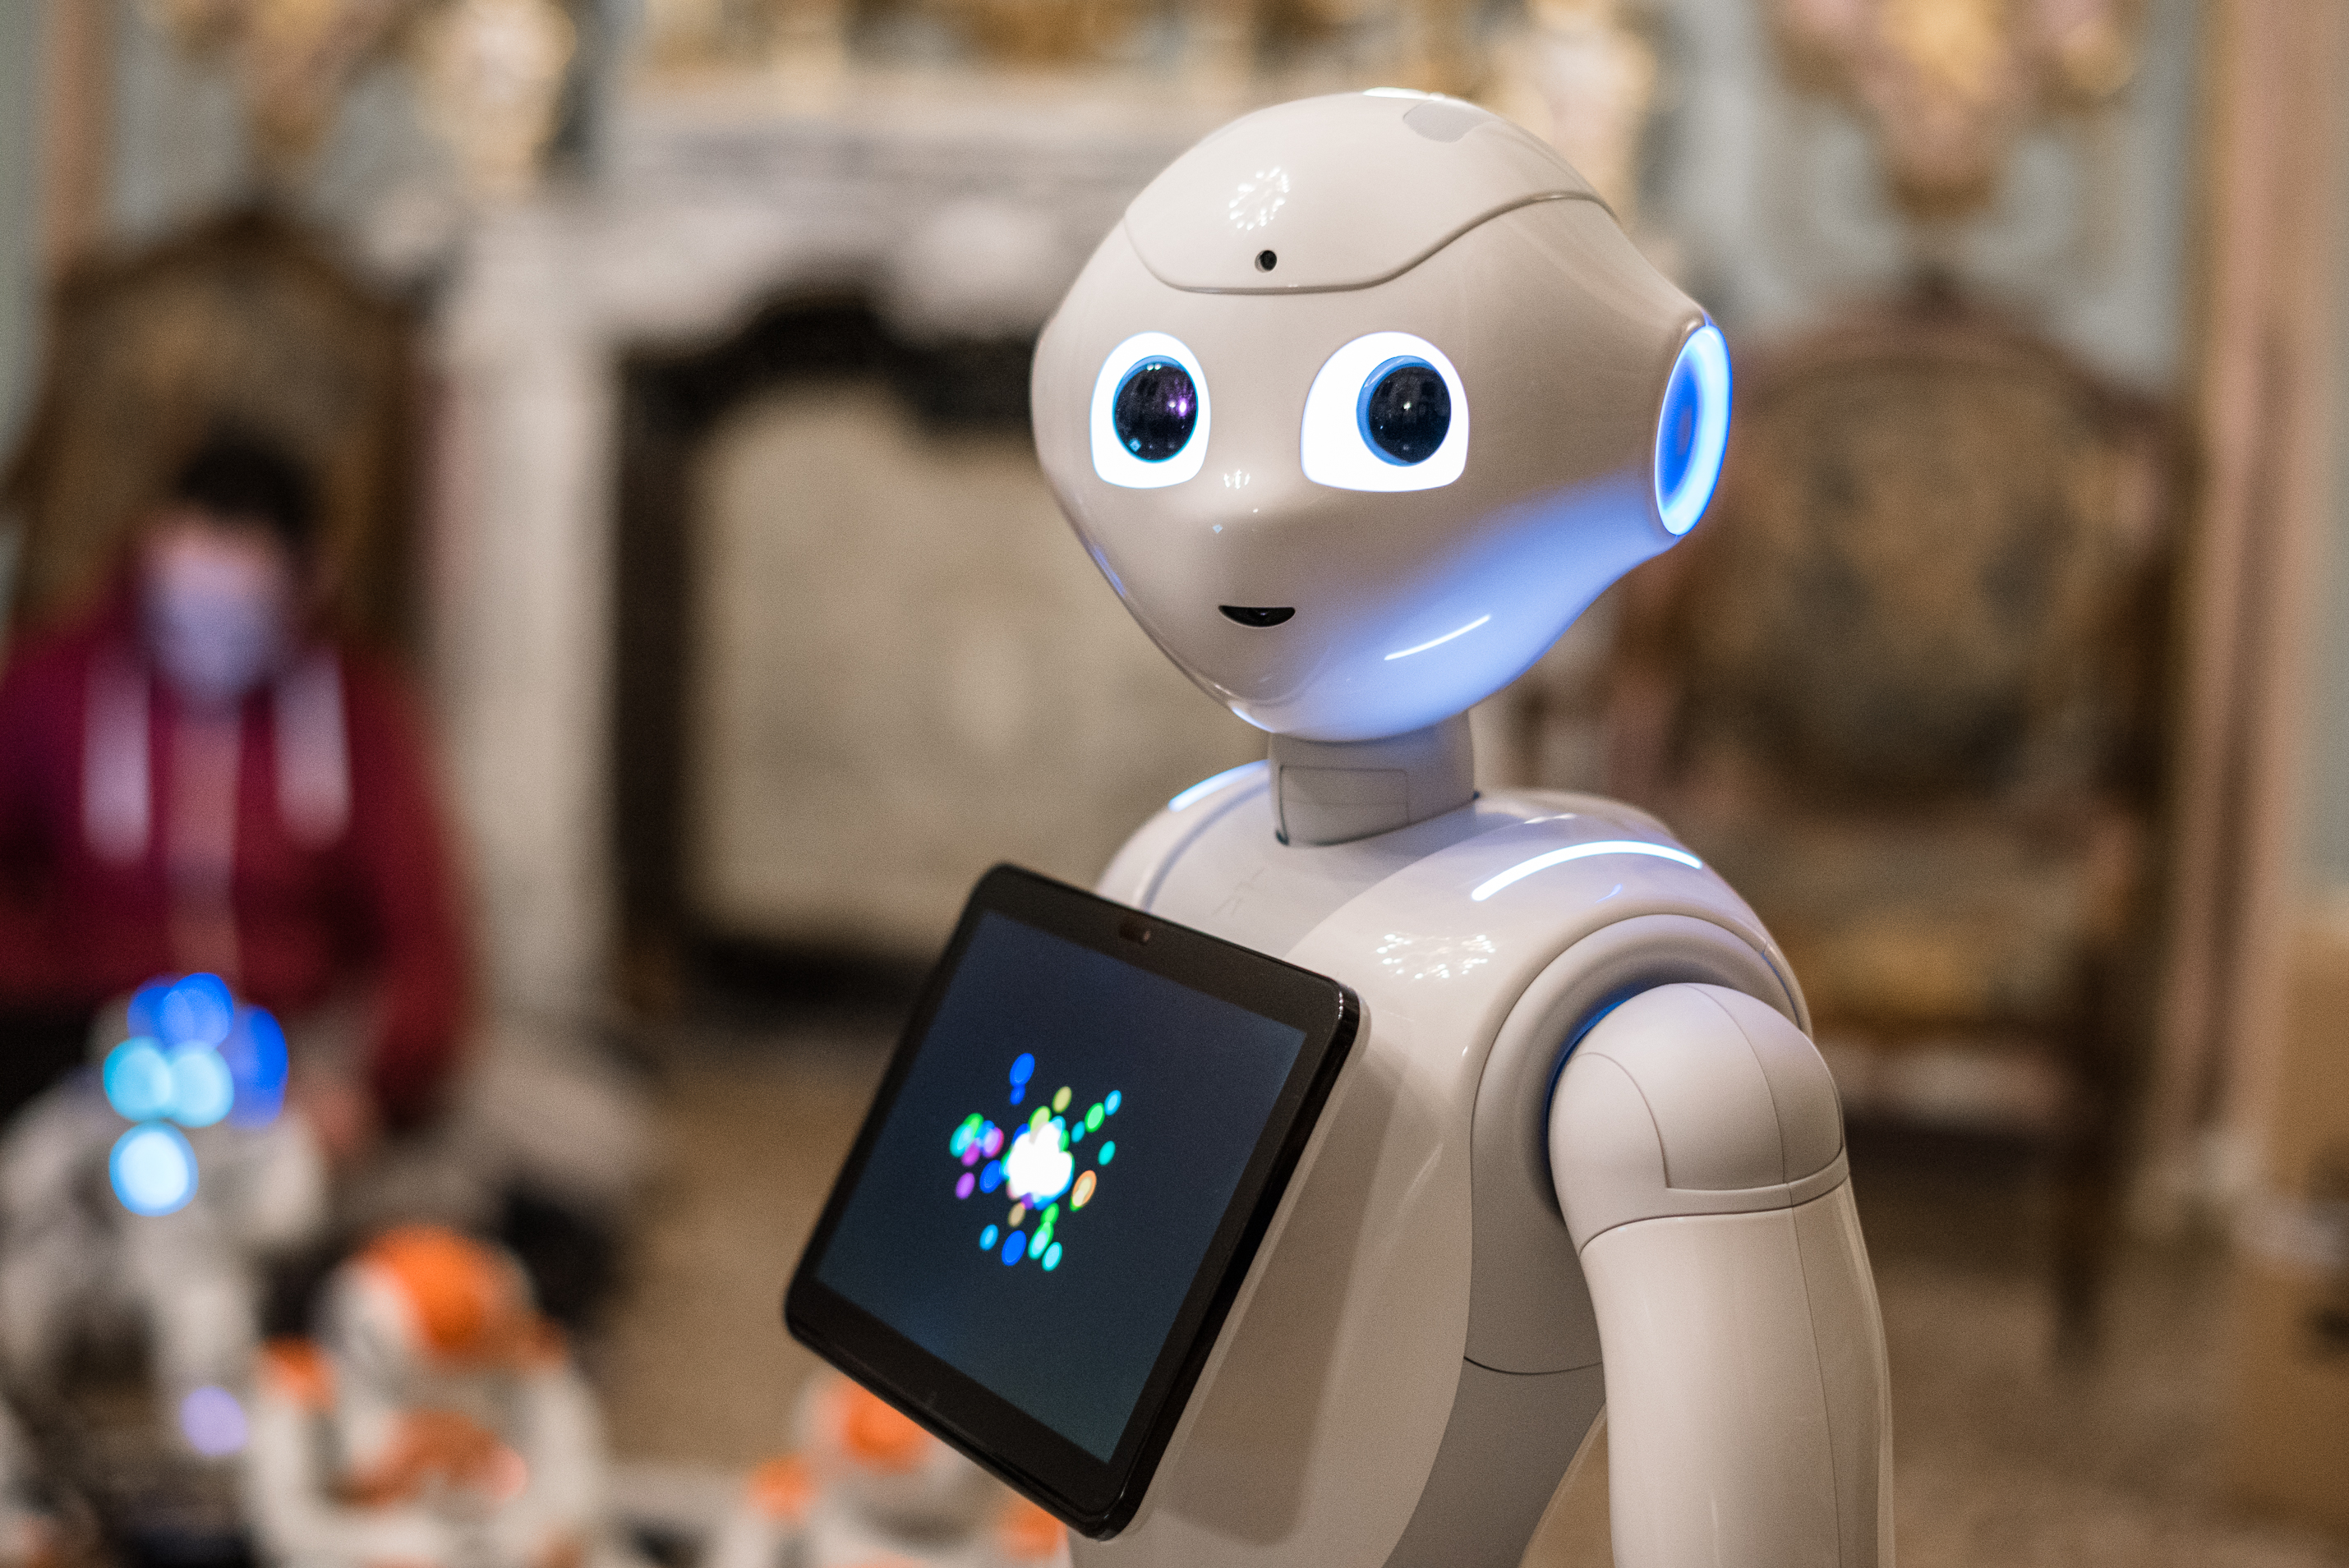
\includegraphics[width=.9\textwidth]{pepper}<1->
		\end{center}
		\end{figure}
\end{columns}
\end{frame}

\begin{frame}
\frametitle{NAO In The Store}
\begin{columns}
	\column{0.5\textwidth}
		Obiettivi:
		\begin{itemize}
			\item<2-> Creare un dialogo con NAO
			\item<3-> Ogni possibile risposta deve risultare in azioni diverse del robot
			\item<4-> Utilizzare i Behavior
		\end{itemize}
	\column{0.5\textwidth}
		\begin{figure}[ht]
		\begin{center}
		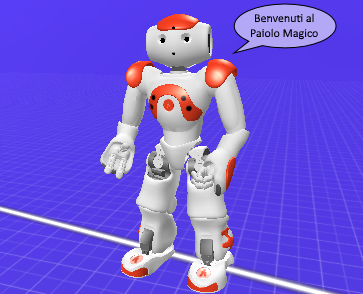
\includegraphics[width=.9\textwidth]{paiolo}<1->
		\end{center}
		\end{figure}
\end{columns}
\end{frame}

\begin{frame}
\frametitle{NAO In The Store}
\begin{columns}
	\column{0.5\textwidth}
		Come:
		\begin{itemize}
			\item<2-> Scegliere il luogo e la situazione in cui si trova NAO
			\item<3-> Provare tutti i Behavior installati e scegliere quelli che si potrebbero utilizzare
			\item<4-> Scrivere il copione con le varie opzioni su carta
			\item<5-> Realizzare il dialogo (blocco Choice)
			\item<6-> Aggiungere i Behavior al dialogo
		\end{itemize}
	\column{0.5\textwidth}
		\begin{figure}[ht]
		\begin{center}
		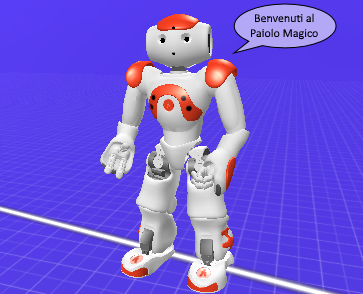
\includegraphics[width=.9\textwidth]{paiolo}<1->
		\end{center}
		\end{figure}
\end{columns}
\end{frame}

\ifx\fulldocument\undefined
\end{document}
\fi
